\subsection{A tree of segments}\label{sec:skeleton}

We begin the proof of \Cref{thm:maintechnical} by supposing that $\calD$ is a class that is closed under identification, but it is not $c$-bounded. The goal is now to show that $\calD$ has a pattern with a $t$-tough pair for all positive integers $t$. Consider an instance where $G$ and $D$ are acyclic.

First, we show that it sufficient to consider a weakly connected acyclic solution $H$ where all vertices have undirected degree at least $3$. To show the minimum degree bound, we contract all edges $uv$ of $H$ (and $G$) where $u$ or $v$ has undirected degree at most $2$. If at least one of $u$ and $v$ is a non-terminal, then such contractions do not influence the feasibility and edge minimality of $H$, and it also does not change the total branch degree of $H$. If both $u$ and $v$ are terminals, then let $H'$ denote the new graph after the contraction, and let us identify $u$ and $v$ in $D$, resulting in the graph $D'$. Since $|D'|=k-1$ and $H$ and $H'$ have the same total branch-degree, we have that if $H$ has total branch degree at least $ck$, then also $H'$ has total branch degree at least $c\cdot (k-1)$. It is therefore sufficient to consider graphs $H$ where all vertices of the undirected graph $\bar H$ have degree at least $3$. (Throughout this section, the notation $\bar{X}$ refers to the undirected graph given by the edges of the graph $X$, where $X$ may be a directed graph or mixed graph.) 

Suppose now that $H$ is disconnected, and let $H_i$ be the connected components of $H$ ($i=1,2,\dots$). For each $H_i$ let $D_i$ be the subgraph of $D$ induced by $T\cap V(H_i)$. Notice that the graphs $D_i$ are a partition of the edges of $D$, where each connected component of $D$ is contained in a single graph $D_i$. Observe that each $H_i$ is an edge-minimal solution for the instance $(G,T\cap V(H_i), D_i)$. Moreover, if $H$ has branch-degree at least $ck$, than at least one among the $H_i$ has branch degree at least $c\cdot|T\cap V(H_i)|$. Therefore we can restrict our attention to weakly connected graphs $H$.


\paragraph*{Defining a tree of segments.}
The skeleton $S$ is a $2$-connected mixed graph that we will build based on an optimum solution $H$ of the instance $(G,T,D)$ of \Dsn where $G$ and $D$ are acyclic.
Suppose now that $H$ is a solution to $(G,T,D)$ that is a connected acyclic graph of minimum degree at least $3$.
We fix a plane embedding of $H$, and add undirected edges to $\bar{H}$ in a greedy manner to create a triangulation of the plane with vertex set $V(H)$; let $H_\Delta$ denote the resulting mixed graph, where the edges of $H$ are directed, and the newly added triangulation edges are undirected.

A \emph{long segment} is a \emph{directed} path of length at least $L$ in $H_\Delta$. A \emph{short segment} is a path of $\bar{H}_\Delta$ (i.e., of arbitrary orientation edges in $H_\Delta$) that consists of at most $L$ edges. A pair of segments $A,B$ are \emph{distant} if for any pair of vertices $a\in A$ and $b\in B$ the distance of $a$ and $b$ in $\bar{H}$ is at least $L$. Our goal is to create a skeleton where the boundary of the so-called \emph{relevant} face consists of $O(k)$ (long and short) segments where the long segments are pairwise distant.

Next, we construct a tree $R$ in $H_\Delta$ consisting of $O(k)$ segments that contains all terminals.

\begin{lemma}\label{lem:maketree}
There is a tree $R$ in $H_\Delta$ that contains all terminals and consists of $O(k)$ segments, such that any pair of long segments of $R$ are distant.
\end{lemma}

\begin{proof}
Initially, we set $R$ to be the edgeless forest with vertex set $T$. We add segments to $R$ using the following insertions, until it becomes connected.

\begin{description}
\item[Insertion 1.] Let $C$ and $C'$ be the closest components of the current graph $R$, that is, the pair of components where $\delta(C,C'):=\min_{u\in V(C), v\in V(C')} \dist_{\bar{H}_\Delta} (u,v)$ is minimized. If $\delta(C,C')\leq 2L$, then let $P$ be a shortest path connecting $C$ and $C'$ in $H_\Delta$. Since $|P|\leq 2L$, we can decompose $P$ into at most two segments, which we add to $R$, connecting $C$ and~$C'$.
\item[Insertion 2.]
Suppose that $R$ is not connected, but Insertion 1 can no longer be applied. A vertex $v$ is a \emph{collaborator} of a component $C$ of $R$ if there is an edge $e$ incident to $v$ that is essential for some demand $tt'$ where $t\in V(C)$ or $t'\in V(C)$. 
Let $v$ be a vertex that collaborates with at least two distinct components. Let $P_v$ and $P'_v$ be directed paths connecting $v$ to these two components. We shortcut the loops of $P_v\cup P'_v$, to find a path $P$ whose internal vertices are outside $N_R$ that connects two distinct neighborhoods $N_C$ and $N_{C'}$. Note that $P$ is the concatenation of at most two directed paths, thus it can be decomposed into at most two short or long segments. If we have two long segments, we also need to separate these with a short segment: let $u$ be the first vertex on the first long segment that is within $\bar{H}$-distance $L$ to the other long segment. We connect $u$ to the last vertex $v$ of the other long segment to which it has distance $L$ using a short segment, and remove the parts of the long segments that fall between $u$ and $v$. Let $P$ be the final path, which now consists of at most $3$ segments, and if it has two long segments, then those are distant. Connecting the endpoints of $P$ to $C$ and $C'$ with short segments, we are able to add at most five segments to $R$ that connect $C$ and~$C'$. 
\end{description}

We claim that applying the above insertions exhaustively leads to a tree that contains all terminals. Observe that after each successful insertion the number of connected components of $R$ decreases by at least one (and no cycles can be created), thus after at most $k-1$ insertions we get a connected tree $R$. In order to show this, we need to show that as long as $R$ is disconnected, there is an insertion that we can apply.

\begin{claim}
If $R$ is disconnected, then at least one of the insertions can be applied.
\end{claim}
\begin{claimproof}
Suppose for the sake of contradiction that Insertion 1 and 2 cannot be applied, but $R$ is still disconnected. It follows that each vertex collaborates with at most one component. If some edge $e$ is essential for demand $t_it_j$ and the terminals $t_i,t_j$ lie in different connected components of $R$, then Insertion 2 can be applied, so suppose that no such edge exists, i.e., for each edge the corresponding demand terminals fall into the same component. Since all edges $e$ of $H$ are essential and $H$ has no isolated vertices, we have that all vertices of $H$ collaborate with at least one component of~$R$.

Let $P_0$ be a path in $\bar H$ connecting the distinct components $C$ and $C'$ of $R$ whose internal vertices are disjoint from $V(R)$: such a path exists because $R$ is a disconnected subgraph of the connected graph $H$. The starting vertex of $P_0$ collaborates with $C$, and its ending vertex collaborates with $C'$, so there must be an edge $e$ along this path whose endpoints collaborate with distinct components. But this contradicts the definition of collaboration, which implies that adjacent vertices collaborate with all components for which the connecting edge is essential.
\end{claimproof}

Notice that each insertion adds at most $5$ new segments to $R$, and we can do at most $k-1$ insertions to reach the final tree $R$, thus the final tree $R$ consists of at most $5k-5$ segments. Moreover, long segments can only be added with Insertion 2 and 3, and each of them adds a long segment outside the current $N_R$, thus the newly added long segments are distant from all earlier long segments. Thus insertions preserve the property that long segments are pairwise distant. This concludes the proof.
\end{proof}


\subsection{Region slicing}\label{sec:Sperner}

We will now slice the plane into smaller regions using segments. We say that a closed region (some connected union of faces of $H_\Delta$) in the plane is \emph{relevant} if it is interior-disjoint from the plane tree $R$.  We work towards the following lemma.

\begin{lemma}[Skeleton Lemma]\label{lem:slicedskeleton}
There is a subgraph $\Skel \subset H_\Delta$ consisting of $O(k)$ segments where the faces of $\Skel$ are relevant and they partition the plane, each face of $\Skel$ has at most $35$ segments on its boundary, and within the subgraph of $\bar{H}$ induced by each face of $\Skel$ any pair of long segments on the face boundary are either subpaths of the same directed path of $H$, or they are distant.
\end{lemma}

The proof of the lemma requires a good separation, which we will prove next. The separator that we prove relies on Sperner's lemma, which can be phrased as follows.

\begin{theorem}[Sperner's lemma]
Let $G$ be an undirected simple plane graph where the vertices are assigned one of three colors (red, green, or blue). Suppose that other than the outer face, the rest of the graph is triangulated. Moreover, suppose that the boundary of the outer face has three marked vertices, $v_1,v_2,v_3$ colored with $1,2,3$, and that each vertex on the boundary is assigned one of the colors of the two marked vertices that enclose it on the boundary. Then $G$ has a triangle whose vertices have three different colors.
\end{theorem}

If $\calF$ is a relevant region bounded by some cycle of $\bar{H}_\Delta$, then let $H^\calF$ and $H^\calF_\Delta$ denote the subgraph of $H$ and $H_\Delta$ consisting of the edges in $\calF$ (including edges on the boundary of $\calF$), respectively.

\begin{lemma}[Separator]\label{lem:sperner_sep}
Let $\calF$ be relevant region of $H$ that is bounded by a cycle $F$ of $\bar{H}_\Delta$ which consists of $s\geq 36$ segments, where long segments are distant in $\bar{H}^\calF$. Then there is a path $P$ in $\calF$ that splits $\calF$ into two regions, $\calF_1$ and $\calF_2$ with boundary cycles $F_1$ and $F_2$ consisting of $s_1$ and $s_2$ segments, so that
\begin{itemize}
\item long segments in $F\cup P=F_1\cup F_2$ are distant,
\item $s_1+s_2\leq s+12$,
\item and $13\leq  s_1,s_2 \leq s-4$.
\end{itemize} 
\end{lemma}

\begin{proof}
We will assign colors to the vertices of $H_\Delta$ that fall in $\calF$. First, we split the boundary cycle $\bar{F}$ into three paths $P_1,P_2,P_3$ of almost equal number of segments, i.e., so that the number of segments on each of these paths have a difference of at most 1. We color the endpoints of the paths with $1,2$ and $3$ so that $P_i$ goes from the point of color $i$ to the point of color $i+1$, where indices are defined modulo $3$. Next, all internal vertices of $P_i$ will be colored by $i$ for each $i=1,2,3$, see Figure~\ref{fig:sperner}.

To color the vertices in the interior of $\calF$, let $v$ be an arbitrary vertex there. Since $v$ is not in $R$, it cannot be a terminal, so it has an essential edge incident to it, which is on some terminal-to terminal path. Let $P_v$ be this directed path connecting two terminals that contains~$v$. Since there are no terminals in the interior of $\calF$, going forward on the path we will eventually exit $\calF$. Before this point, there will be a first vertex $w$ of $P$ after $v$ that is of distance at most $L$ to some point $b\in V(F)$, that is, either $\dist{\bar{H}_\Delta^\calF}(v,b)\leq L$ and $v=w$, or $\dist_{\bar{H}^\calF}(w,b)= L$ and $\max_{x\in P[v,w)}\dist_{\bar{H}_\Delta^\calF}(x,V(F))>L$. (If there are multiple vertices $b\in V(F)$ at minimum distance to $w$ in $\bar{H}_\Delta^\calF$, then we choose an arbitrary such vertex $b$). We assign to $v$ the color that we have assigned to $b$. Notice that we have a path $Q$ consisting of a directed path (a subpath of $P_v$) and a short segment that connects $v$ to $b$, and $Q$ is distant from all long segments of $V(F)$.

\begin{figure}[t]
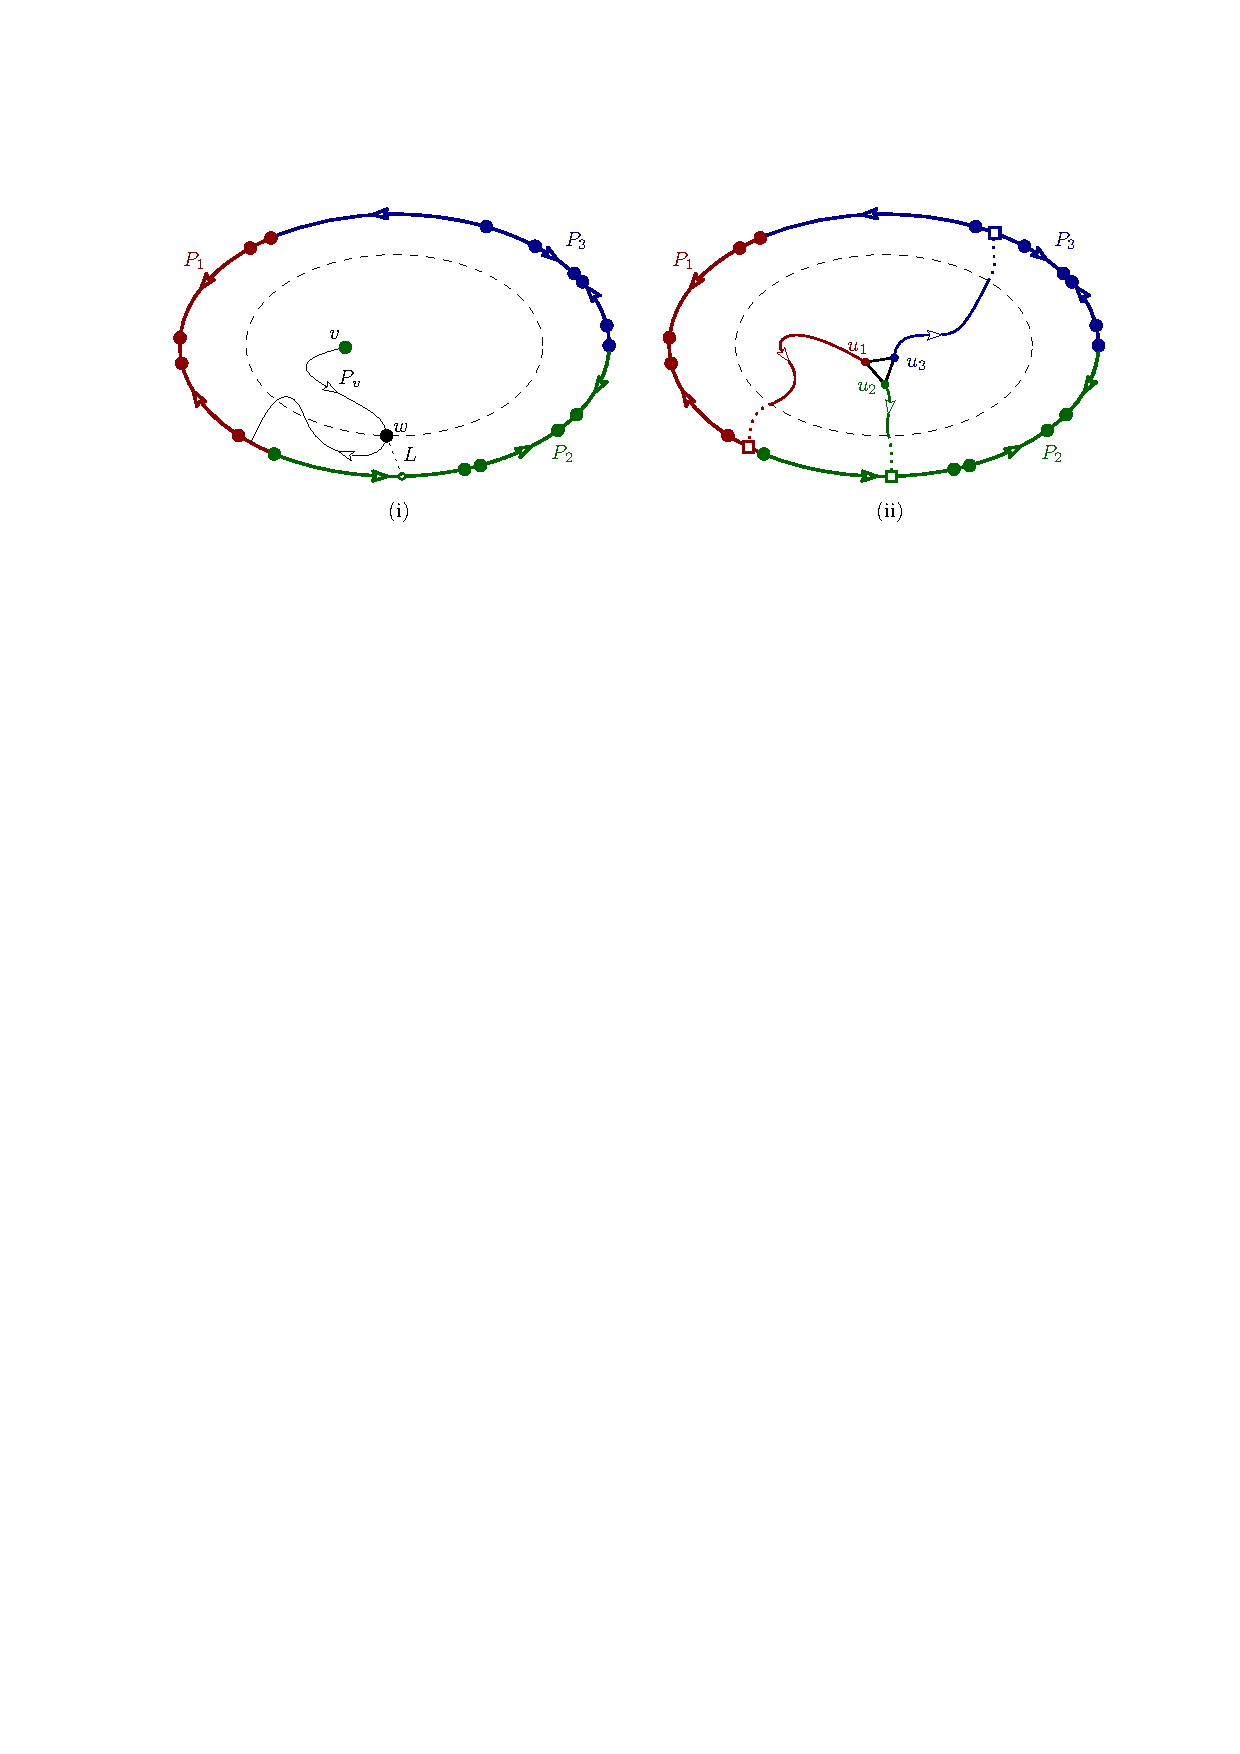
\includegraphics[width=\textwidth]{sperner.pdf}
\caption{(i) Coloring segments on the boundary of the region $\calF$. Long segments are denoted with an arrow. The color of vertex $v$ is defined using a path $P_v$ that arrives in the $L$-neighborhood of $\bd\calF$. (ii) Applying Sperner's lemma in the coloring. Two of the landing vertices in $\bd\calF$ (denoted by empty squares) will be from distant segments along $\bd\calF$.}\label{fig:sperner}
\end{figure}

By Sperner's lemma there is a triangle $u_1u_2u_3$ in this coloring where $u_i$ has color $i$. Let $Q_i$ be the path from $u_i$ to the boundary point $b_i\in V(P_i)$ that we used to assign color $i$ to $u_i$. Since the paths $P_i$ have at least $\lfloor s/3 \rfloor$ segments, we have that there is a pair $b',b''$ among $b_1,b_2,b_3$ such that  along $F$ there are at least $\lfloor s/3 \rfloor$ complete segments between them (and up to two partial segments). Let $u',u''\in \{u_1,u_2,u_3\}$ and $Q',Q''\in \{Q_1,Q_2,Q_3\}$ be the starting points and paths corresponding to $b'$ and $b''$. Consider the path that is the concatenation of $Q'$, the edge $b'b''$, and $Q''$. If both $Q'$ and $Q''$ contain long segments attached to $u'$ and $u''$, then the path can be shortcut in the middle with a short segment to ensure that they remain distant from each other: let $u$ be the first vertex on the first long segment that is within $\bar{H}$-distance $L$ to the other long segment. We connect $u$ to the last vertex $v$ of the other long segment to which it has distance $L$ using a short segment, and remove the parts of the long segments that fall between $u$ and $v$.

Let $P$ be the resulting path connecting $b'$ and $b''$, and let $\calF_1$ and $\calF_2$ be the regions that we get by splitting $\calF$ with $P$. By construction, the resulting path consists of at most $5$ segments, and long segments in $F\cup P$ are pairwise distant. Note that the vertices $b'$ and $b''$ may be internal vertices of some segment of $F$, and in such a case the corresponding segment will be counted both in $F_1$ and $F_2$. We are also counting the at most $5$ segments of $P$ both times. Thus we have that $s_1+s_2\leq s+2+2\cdot 5 = s+12$. Since $P$ has at least one segment, we have that $\min(s_1,s_2)\geq \lfloor s/3 \rfloor + 1\geq 13$ since $s\geq 36$. Taking into account the partial segments, the upper bound can be written as $\max(s_1,s_2)\leq s-\lfloor s/3 \rfloor + 2 + 5 \leq 2s/3 + 8\leq s-4$, since $s\geq 36$.
\end{proof}

We can use this separator to prove Lemma~\ref{lem:slicedskeleton}, but first let us consider a walk along the boundary of the unbounded face of the plane tree $R$. Notice that the walk uses each edge of $R$ twice, once in each direction. Additionally, whenever we encounter a branching vertex (a vertex of degree at least $3$) of $R$ that is an interior vertex of the segment we have been walking along, then we slice the current segment into two smaller segments at $v$, resulting in two (short or long) segments. As a result, we end up with a walk that consists of the original $O(k)$ segments, plus at most the number of branching vertices of $R$, which is at most $O(k)$, as there are at most $O(k)$ leaves in $R$. Consequently, the walk has at most $O(k)$ segments.

\begin{proof}[Proof of Lemma~\ref{lem:slicedskeleton}]
If the walk around $R$ consists of at most $35$ segments, then we set $\Skel=R$; this has all the desired properties. Otherwise, we recursively slice the region outside $R$ into smaller regions using Lemma~\ref{lem:sperner_sep}, until all regions have at most $35$ segments on their boundary, using the following procedure. 

For a partition $\calP=\{\calF_1,\dots,\calF_t\}$ of the plane where each $\calF_i$ is a non-empty union of faces of $H_\Delta$ and where $F_i$ has $s_i$ boundary segments, we define the potential function \[f(\calP)=\sum_{i=1}^t s_i -13t.\]
Notice that the contribution of region $\calF_i$ to $f(\calP)$ is $s_i-13$. By Lemma~\ref{lem:sperner_sep}, for any region $\calF_i$ appearing throughout the slicing we have $s_i\geq 13$, therefore each region contributes a non-negative integer to $f$. It follows that $f(\calP)\geq 0$ for all partitions $\calP$ that appear in the slicing.

If $F$ is the region boundary of an element of $\calP$ with $s\geq 36$ segments on its boundary, then by Lemma~\ref{lem:sperner_sep}, after the slicing it will be replaced by two regions, and the total number of segments on region boundaries increase by at most $12$. Therefore in the potential function $f$ the number $t$ increases by one, while the segment sum increases by at most $12$. Thus if $\calP'$ is the new partition we get by applying Lemma~\ref{lem:sperner_sep} on $F$, then we have
\[f(\calP')\leq f(\calP)+12-13 = f(\calP)-1.\]
Thus the potential is decreasing in each step. Initially we have a singleton partition with value $O(k)$, and we know that the potential remains non-negative, thus there can be at most $O(k)$ steps. It follows that $\Skel$ consists of $O(k)$ regions, each of which has $O(1)$ segments on their boundary. The long segments of any of the faces $\calF$ in $\Skel$ are either on the same directed path of the original solution $H$, or they are distant inside $\bar{H}^\calF_\Delta$. Indeed, this property is true for the initial singleton partition, the distances are preserved by the slicing, and the distance is not shortened when restricting to a subgraph defined by some region $\calF$.
\end{proof}